\documentclass[norsk,a4paper,12pt]{article}
\usepackage[utf8]{inputenc}
\usepackage{graphicx} %for å inkludere grafikk
\usepackage{verbatim} %for å inkludere filer med tegn LaTeX ikke liker
\usepackage{tabularx}
\usepackage{booktabs}
\usepackage{amsmath}
\usepackage{float}
\usepackage{color}
\usepackage{listings}
\usepackage{hyperref}

\lstset{language=c++}
\lstset{basicstyle=\small}
\lstset{backgroundcolor=\color{white}}
\lstset{frame=single}
\lstset{stringstyle=\ttfamily}
\lstset{keywordstyle=\color{red}\bfseries}
\lstset{commentstyle=\itshape\color{blue}}
\lstset{showspaces=false}
\lstset{showstringspaces=false}
\lstset{showtabs=false}
\lstset{breaklines}
\lstset{postbreak=\raisebox{0ex}[0ex][0ex]{\ensuremath{\color{red}\hookrightarrow\space}}}
\usepackage{titlesec}

\setcounter{secnumdepth}{4}

\titleformat{\paragraph}
{\normalfont\normalsize\bfseries}{\theparagraph}{1em}{}
\titlespacing*{\paragraph}
{0pt}{3.25ex plus 1ex minus .2ex}{1.5ex plus .2ex}


\title{PH4603 - Soft Condensed Matter Physics\\\vspace{2mm} \Large{Homework 1}}
\author{\large Even Marius Nordhagen}
\date\today
\begin{document}

\maketitle

\section*{Problem 1}
The Lennard-Jones potential is given by
\begin{equation}
V(r)=4\epsilon\Bigg[\bigg(\frac{\sigma}{r}\bigg)^{12}-\bigg(\frac{\sigma}{r}\bigg)^6\Bigg]
\end{equation}

Equilibrium separation is the distance between the atoms at which the force on each atom is zero, so firstly we need to find an expression of the force. For that the relation
\begin{equation}
F(r)=-\frac{d}{dr}\Big(V(r)\Big)
\end{equation}
from electrostatics is useful:
$$F(r)=-4\epsilon\Bigg[12\bigg(\frac{\sigma}{r}\bigg)^{11}\cdot-\frac{\sigma}{r}-6\bigg(\frac{\sigma}{r}\bigg)^5\cdot-\frac{\sigma}{r}\Bigg]$$
\begin{equation}
\label{eq:force}
=24\epsilon\Bigg[2\bigg(\frac{\sigma}{r}\bigg)^{12}-\bigg(\frac{\sigma}{r}\bigg)^6\Bigg]\frac{1}{r}
\end{equation}
where the chain rule is used twice. Secondly we need to find the distance between the atoms where no force is acting, so we set the force equal to zero. It gives
$$2\bigg(\frac{\sigma}{r}\bigg)^{12}=\bigg(\frac{\sigma}{r}\bigg)^6$$
$$2\bigg(\frac{\sigma}{r}\bigg)^6=1$$
\begin{equation}
\Rightarrow \quad\underline{r_0=2^{1/6}\sigma}
\end{equation}
\newpage

We were also asked to find the minimum force required to separate the atoms, which needs to be stronger than the strongest attractive force. The repulsive force is defined as the positive force direction, and the strongest attractive force is therefore where the force is at its minimum. The extremal points are found where the derivative is zero:
$$\frac{\partial F(r)}{\partial r}=24\epsilon\bigg[-26\frac{\sigma^{12}}{r^{14}}+7\frac{\sigma^6}{r^8}\bigg]=0$$
$$\Rightarrow \quad26\frac{\sigma^{12}}{r^{14}}=7\frac{\sigma^6}{r^8}$$
\begin{equation}
\Rightarrow \quad r_1=\bigg(\frac{26}{7}\bigg)^{1/6}\sigma
\end{equation}
So this is the distance where the attraction force is at its minimum. Some people may prefer to calculate the second derivative to ensure that the extremal point is a minimum point, but instead I decided to plot the graph, see Figure (\ref{fig:LJforce}). We find the force by inserting into Equation (\ref{eq:force}), and obtain
\begin{equation}
F(r_1)=24\epsilon\Bigg[2\bigg(\frac{7^2}{26^2}\bigg)-\frac{7}{26}\Bigg]\bigg(\frac{7}{26}\bigg)^{1/6}\frac{1}{\sigma}=\underline{-\frac{144}{13}\bigg(\frac{7}{26}\bigg)^{7/6}\frac{\epsilon}{\sigma}}
\end{equation}
\begin{figure}[!htbp]
\centering
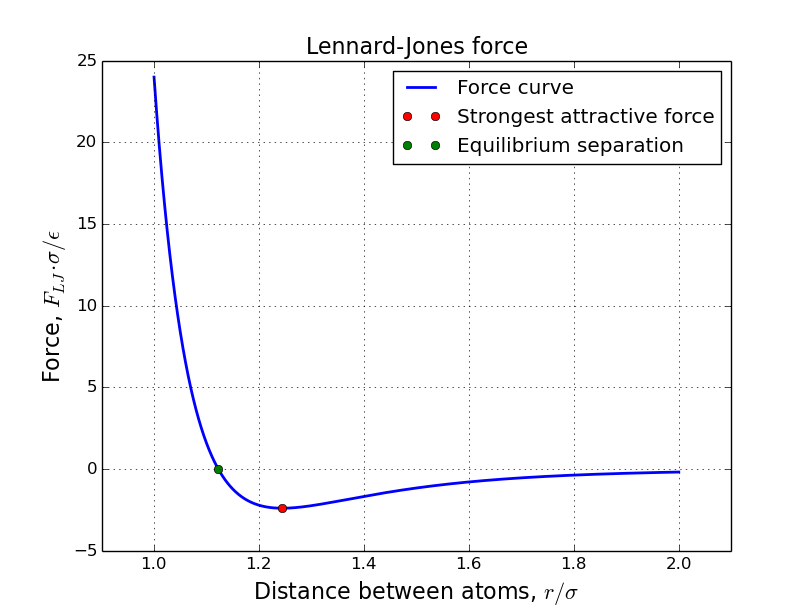
\includegraphics[width=100mm]{figure_1.png}
\caption{The force plotted when the dimensionless variable $r/\sigma$ goes from 1 to 2. $r_0$ and $r_1$ are marked on the curve. \label{fig:LJforce}}
\end{figure}

\section*{Problem 2}
\subsection*{Covalent bonds}
In general atoms want to have the maximum number of electron in the Valence band because it makes the atom stable. In a molecule, the atoms can "share" electrons, which make the atoms stable and satisfied. The result is that the energy of the molecule is lower than when the atoms are separated, resulting in a strong bond which only can be broken by adding the lowering energy. 

\subsection*{Ionic bonds}
Ionic bonds are, as the name implies, bonds between ions. Ions are in fact charged atoms, so the interaction is given by the Coulomb potential
\begin{equation}
U_c=\frac{q_1q_2}{4\pi\epsilon_0r}
\end{equation}
where $q_1$ and $q_2$ are the charges and $r$ is the distance between them.

\subsection*{Hydrogen bonds}
Hydrogen bonds occur when hydrogen atoms are covalently bonded to a negative ion, such as oxygen or nitrogen. Then we get a molecule with a positive part (the hydrogen part) and a negative part, which can interact with similar molecules. An everyday example of a such molecule is $H_2O$, still water, which definitely form hydrogen bonds. The bond is the reason why the water prefer to stick together, like in drops, and the reason why it really hurts when you try to plunge into water, but fail. The hydrogen bond is weak compared to the bonds mentioned above.

\section*{Problem 3}
The general expression for the probability in the canonical system is
\begin{equation}
P(s)=\frac{1}{Z}\exp{[-E(s)/kT]}
\end{equation}
but how do we turn the probability to a function of $E$? We have that
\begin{equation}
P(E)=\frac{\Omega(E)}{Z}\exp{[-E/kT}].
\label{eq:prob_energy}
\end{equation}
Further we know that the entropy is given by the famous entropy formula
\begin{equation}
S=k\ln\Omega(E)
\end{equation}
which leads to
\begin{equation}
\Omega=\exp{[S/k]}.
\end{equation}
By inserting into Equation(\ref{eq:prob_energy}) we obtain
\begin{equation*}
P(E)=\frac{1}{Z}\exp{[S/k]}\exp{[-E/kT]}=\frac{1}{Z}\exp{[-(E-TS)/kT]}
\end{equation*}
\begin{equation}
=\underline{\frac{1}{Z}\exp{[-F/kT]}}
\end{equation}


\section*{Problem 4}
In the canonical system the average of a quantity $Q_i$ is given by
\begin{equation}
\langle Q_i \rangle = \sum_iQ_ip(E_i)
\end{equation}
We can of course calculate the average energy by this formula:
$$\langle E\rangle = \sum_sE(s)p\big(E(s)\big)$$
From the previous problem we know the expression of the probability, and we therefore obtain
$$\langle E \rangle = \frac{1}{Z}\sum_s E(s) \exp\big[{-\beta E(s)}\big]$$
The trick now is recognize that the sum is the derivative of a sum
\begin{equation}
\sum_sE(s)\exp{[-\beta E(s)]}=-\frac{\partial}{\partial \beta}\sum_s\exp{[-\beta E(s)]}=-\frac{\partial Z}{\partial \beta}
\end{equation}
where the partial function given in the problem description is used. Finally we obtain
\begin{equation}
\underline{\langle E\rangle=-\frac{1}{Z}\frac{\partial Z}{\partial\beta}}
\end{equation}
\end{document}
